%
% ---------------------------------------------------------------
% Copyright (C) 2012-2018 Gang Li
% ---------------------------------------------------------------
%
% This work is the default powerdot-tuliplab style test file and may be
% distributed and/or modified under the conditions of the LaTeX Project Public
% License, either version 1.3 of this license or (at your option) any later
% version. The latest version of this license is in
% http://www.latex-project.org/lppl.txt and version 1.3 or later is part of all
% distributions of LaTeX version 2003/12/01 or later.
%
% This work has the LPPL maintenance status "maintained".
%
% This Current Maintainer of this work is Gang Li.
%
%

\documentclass[
 size=14pt,
 paper=smartboard,  %a4paper, smartboard, screen
 mode=present, 		%present, handout, print
 display=slides, 	% slidesnotes, notes, slides
 style=tuliplab,  	% TULIP Lab style
 pauseslide,
 fleqn,leqno]{powerdot}


\usepackage{cancel}
\usepackage{caption}
\usepackage{stackengine}
\usepackage{smartdiagram}
\usepackage{attrib}
\usepackage{amssymb}
\usepackage{amsmath} 
\usepackage{amsthm} 
\usepackage{mathtools}
\usepackage{rotating}
\usepackage{graphicx}

\usepackage{boxedminipage}
\usepackage{rotate}
\usepackage{calc}
\usepackage[absolute]{textpos}
\usepackage{psfrag,overpic}
\usepackage{fouriernc}
\usepackage{pstricks,pst-3d,pst-grad,pstricks-add,pst-text,pst-node,pst-tree}
\usepackage{moreverb,epsfig,subfigure}
\usepackage{color}
\usepackage{booktabs}
\usepackage{etex}
\usepackage{breqn}
\usepackage{multirow}
\usepackage{natbib}
\usepackage{bibentry}
\usepackage{gitinfo2}
\usepackage{siunitx}
\usepackage{nicefrac}
%\usepackage{geometry}
%\geometry{verbose,letterpaper}
\usepackage{media9}
\usepackage{animate}
%\usepackage{movie15}
\usepackage{auto-pst-pdf}

\usepackage{breakurl}
\usepackage{fontawesome}
\usepackage{xcolor}
\usepackage{multicol}



\usepackage{verbatim}
\usepackage[utf8]{inputenc}
\usepackage{dtk-logos}
\usepackage{tikz}
\usepackage{adigraph}
%\usepackage{tkz-graph}
\usepackage{hyperref}
%\usepackage{ulem}
\usepackage{pgfplots}
\usepackage{verbatim}
\usepackage{fontawesome}


\usepackage{todonotes}
% \usepackage{pst-rel-points}
\usepackage{animate}
\usepackage{fontawesome}

\usepackage{listings}
\lstset{frameround=fttt,
frame=trBL,
stringstyle=\ttfamily,
backgroundcolor=\color{yellow!20},
basicstyle=\footnotesize\ttfamily}
\lstnewenvironment{code}{
\lstset{frame=single,escapeinside=`',
backgroundcolor=\color{yellow!20},
basicstyle=\footnotesize\ttfamily}
}{}


\usepackage{hyperref}
\hypersetup{ % TODO: PDF meta Data
  pdftitle={Presentation Title},
  pdfauthor={Gang Li},
  pdfpagemode={FullScreen},
  pdfborder={0 0 0}
}


% \usepackage{auto-pst-pdf}
% package to show source code

\definecolor{LightGray}{rgb}{0.9,0.9,0.9}
\newlength{\pixel}\setlength\pixel{0.000714285714\slidewidth}
\setlength{\TPHorizModule}{\slidewidth}
\setlength{\TPVertModule}{\slideheight}
\newcommand\highlight[1]{\fbox{#1}}
\newcommand\icite[1]{{\footnotesize [#1]}}

\newcommand\twotonebox[2]{\fcolorbox{pdcolor2}{pdcolor2}
{#1\vphantom{#2}}\fcolorbox{pdcolor2}{white}{#2\vphantom{#1}}}
\newcommand\twotoneboxo[2]{\fcolorbox{pdcolor2}{pdcolor2}
{#1}\fcolorbox{pdcolor2}{white}{#2}}
\newcommand\vpspace[1]{\vphantom{\vspace{#1}}}
\newcommand\hpspace[1]{\hphantom{\hspace{#1}}}
\newcommand\COMMENT[1]{}

\newcommand\placepos[3]{\hbox to\z@{\kern#1S
        \raisebox{-#2}[\z@][\z@]{#3}\hss}\ignorespaces}

\renewcommand{\baselinestretch}{1.2}


\newcommand{\draftnote}[3]{
	\todo[author=#2,color=#1!30,size=\footnotesize]{\textsf{#3}}	}
% TODO: add yourself here:
%
\newcommand{\gangli}[1]{\draftnote{blue}{GLi:}{#1}}
\newcommand{\shaoni}[1]{\draftnote{green}{sn:}{#1}}
\newcommand{\gliMarker}
	{\todo[author=GLi,size=\tiny,inline,color=blue!40]
	{Gang Li has worked up to here.}}
\newcommand{\snMarker}
	{\todo[author=Sn,size=\tiny,inline,color=green!40]
	{Shaoni has worked up to here.}}

%%%%%%%%%%%%%%%%%%%%%%%%%%%%%%%%%%%%%%%%%%%%%%%%%%%%%%%%%%%%%%%%%%%%%%%%
% title
% TODO: Customize to your Own Title, Name, Address
%
\title{What's Cooking}
\author{
   Jincai Ma
\\
\\Xi'an Shiyou University}
\date{\today}


% Customize the setting of slides
\pdsetup{
% TODO: Customize the left footer, and right footer
rf=\href{http://www.tulip.org.au}{
Last Changed by: \textsc{\gitCommitterName}\ \gitVtagn-\gitAbbrevHash\ (\gitAuthorDate)
},
cf={What's Cooking},
}


\begin{document}

\maketitle

%\begin{slide}{Overview}
%\tableofcontents[content=sections]
%\end{slide}


%%==========================================================================================




%%==========================================================================================
%%
\begin{slide}{Introduction}
\begin{center}

{
\begin{itemize}
\item 
Use recipe ingredients to categorize the cuisine.\\
Given the name of the condiment, predict the cuisine to which the dish belongs.
\item In the dataset,  including the recipe ID, the dish, and the list of ingredients for each recipe (variable length).The data is stored in JSON format. \\
1.train.json- A training set that contains the recipe ID, dish type, and ingredient list
2.test.json- A test set containing a recipe ID and a list of ingredients
3.sample_submission.csv-Properly formatted sample submission document
\end{itemize}
}

\end{center}
\bigskip
\begin{center}

\end{center}
\bigskip

%%==========================================================================================

%%==========================================================================================

\end{slide}
%%
%%==========================================================================================



%%
\begin{slide}{Data Import And Introduction}
  \begin{center}

    {
      \begin{itemize}
        \item
        Import the JSON file with Pandas:
        We can get the data set of dish names, including 39774 training data and 9944 test samples.
        \item To see the distribution of our data set and the total variety of dishes, we printed out some of the data samples.
      \end{itemize}  
      \begin{figure}
        \centering
        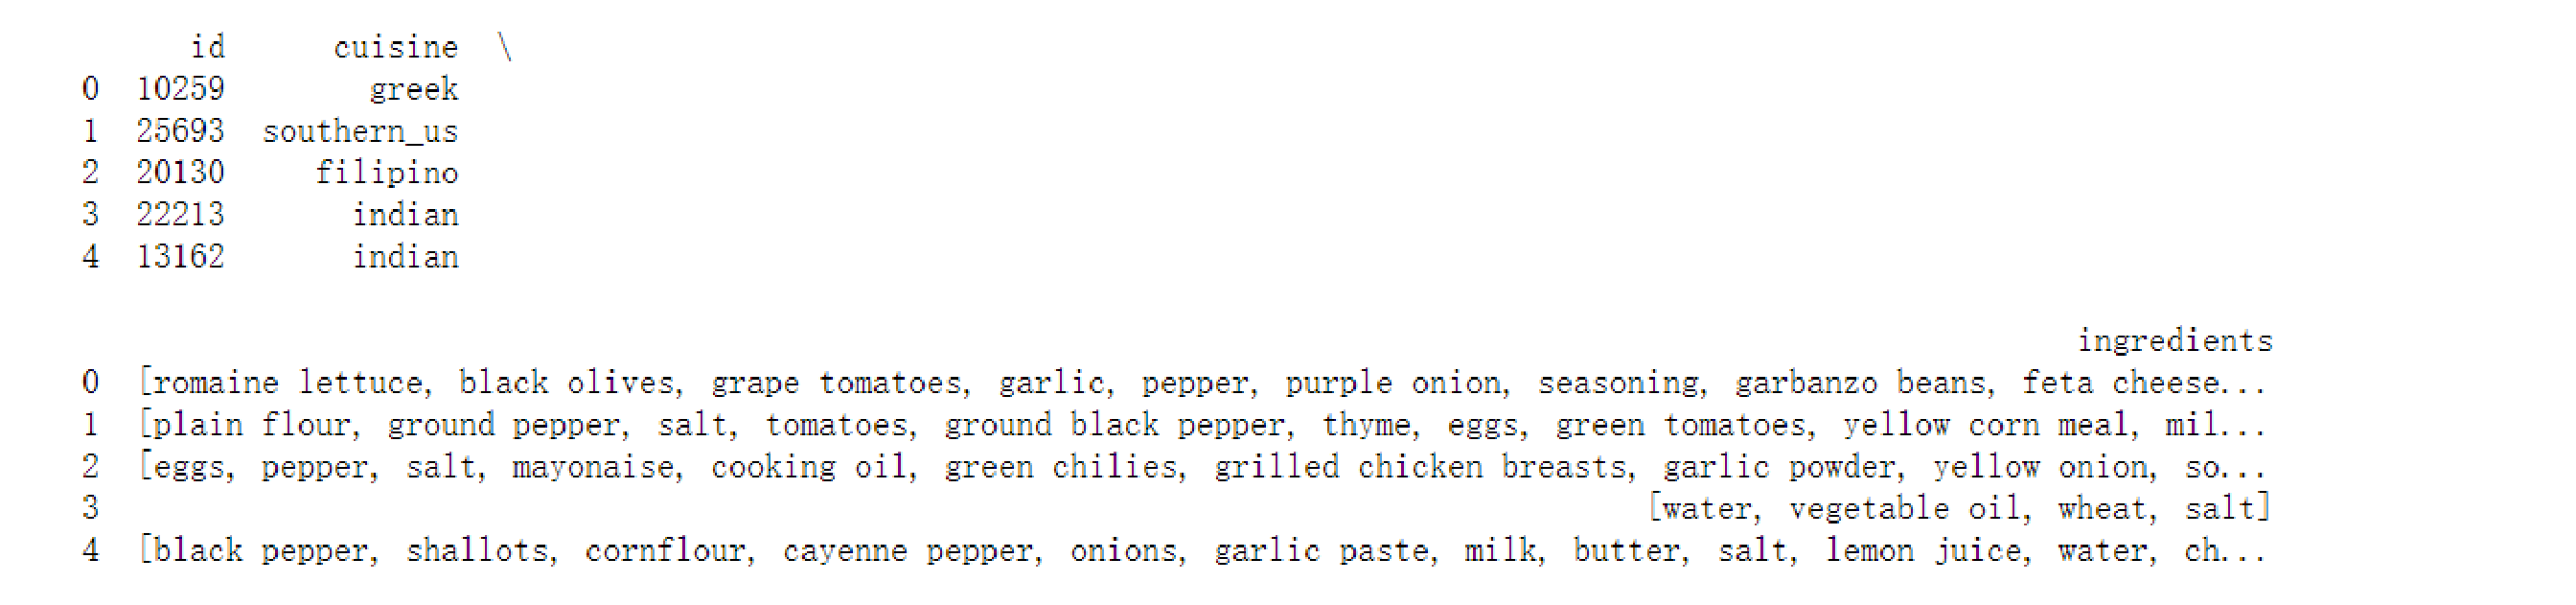
\includegraphics[width=0.9\textwidth]{pic01/a.eps}
        \begin{itemize}
          \item
          Total dish classification\\
          There are 20 dishes in total, which are:
          ['brazilian' 'british' 'cajun_creole' 'chinese' 'filipino' 'french'
           'greek' 'indian' 'irish' 'italian' 'jamaican' 'japanese' 'korean'
           'mexican' 'moroccan' 'russian' 'southern_us' 'spanish' 'thai'
           'vietnamese']
          
        \end{itemize}  
      \end{figure}
    

        
       
    }
    \end{center}
    \bigskip
    \begin{center}
    
    \end{center}
    \bigskip

%%==========================================================================================


%%==========================================================================================
\end{slide}
%%
%%==========================================================================================

%%==========================================================================================
%%
\begin{slide}{Analyze Data}
  \begin{center}

    {
      \begin{itemize}
      
        \item The data set is divided into Features and Target Variables.\\
        \item Features:'ingredients', we were given the names of the ingredients contained in each dish.
        Target variable:'cuisine', is the classification of cuisines that we want to predict.
        \item Extract the Feature of training data set into train_integredients variable
              Extract the Target Variables into the train_Targets variable
      \end{itemize} 
      \begin{figure}
        \centering
        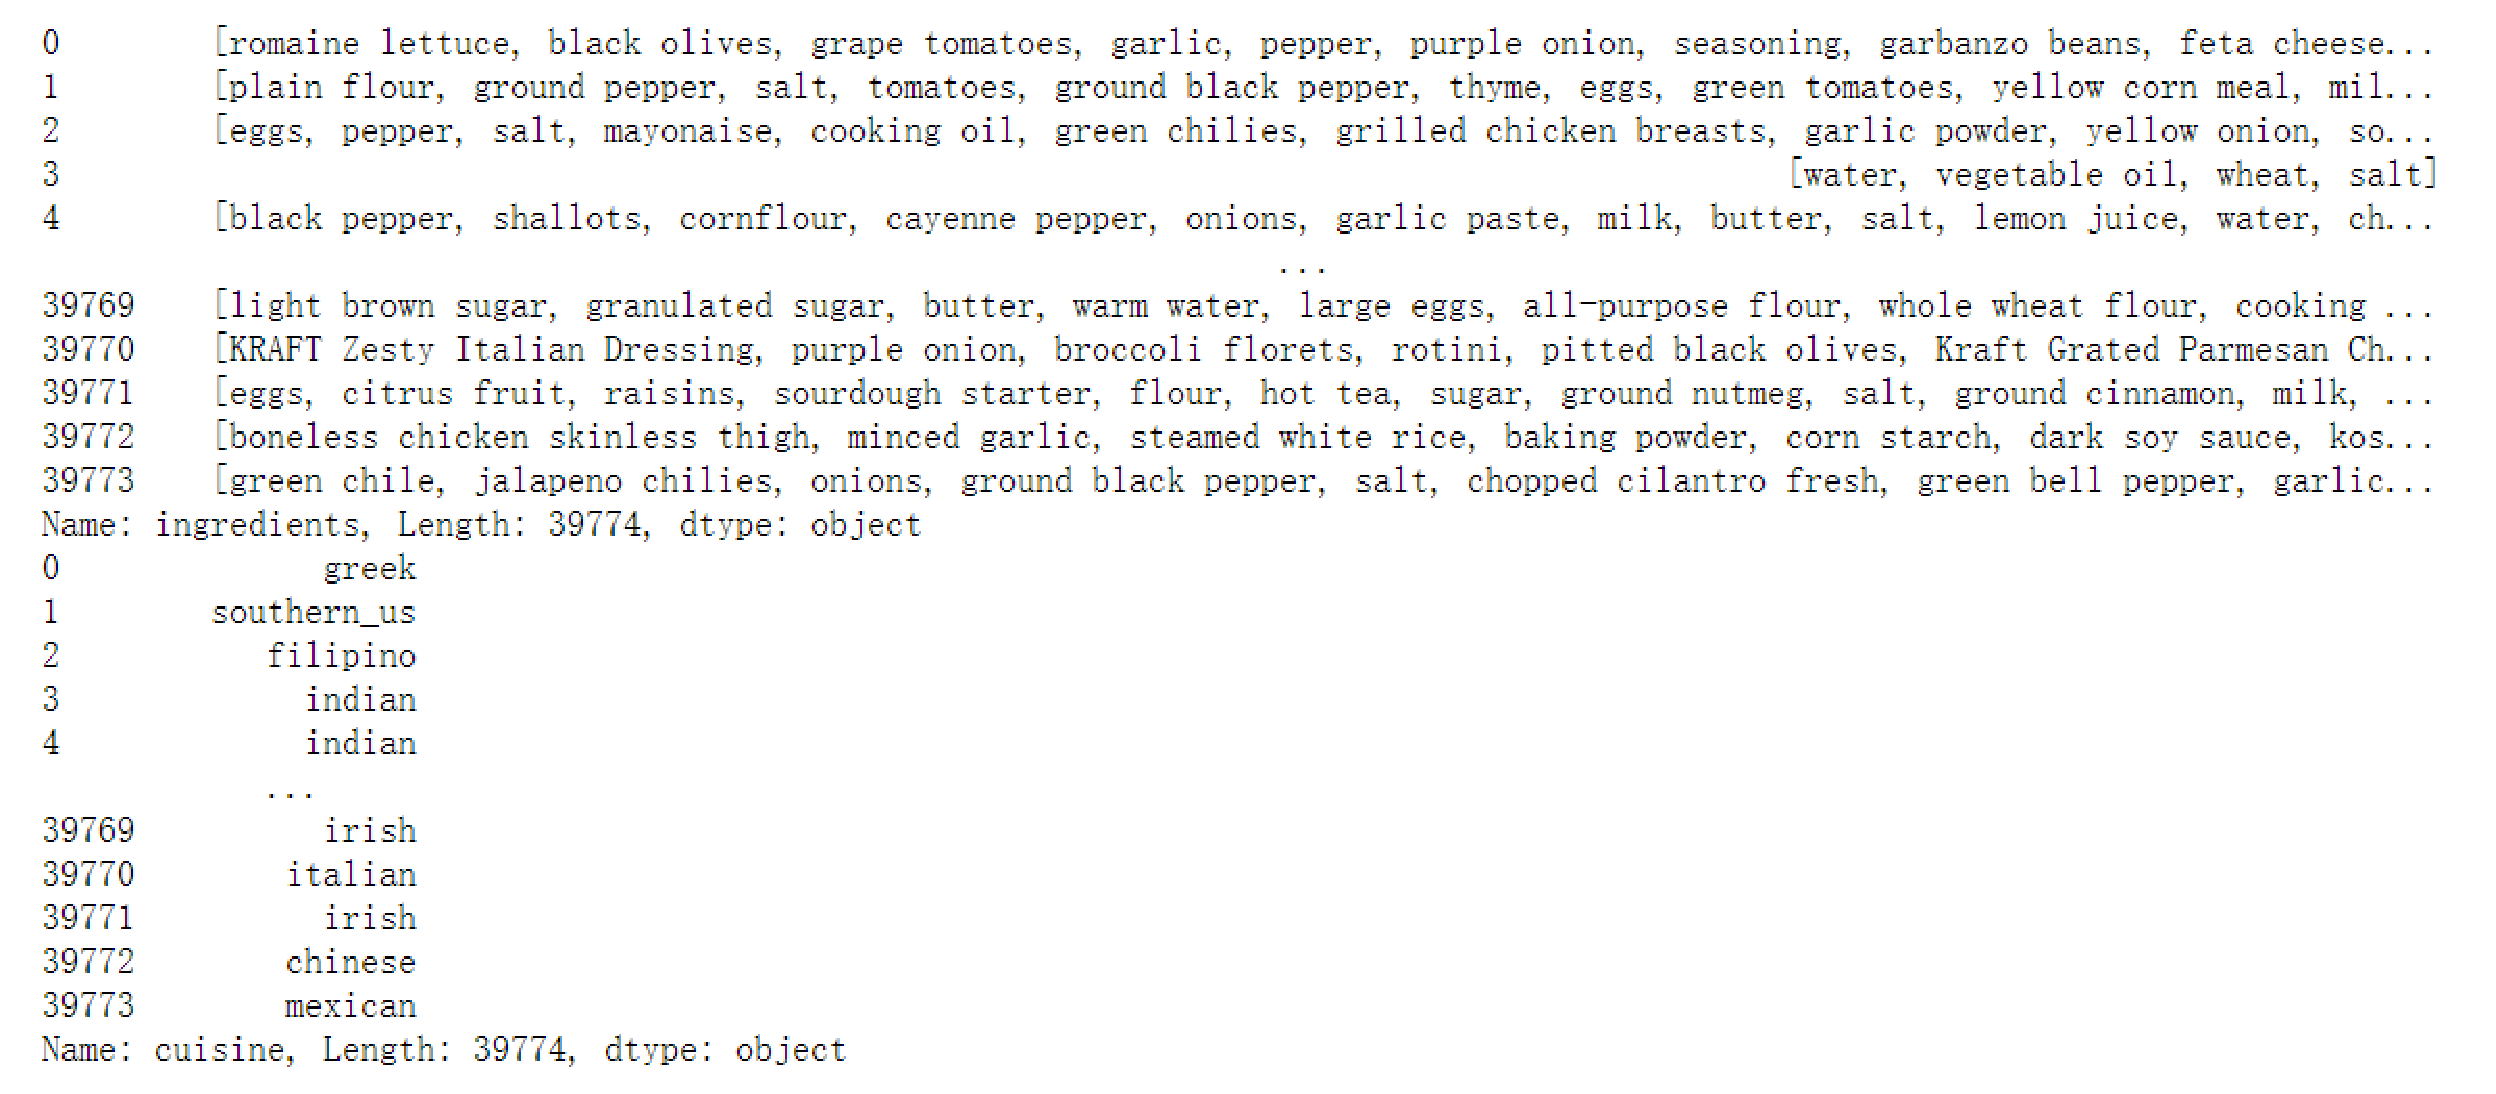
\includegraphics[width=0.7\textwidth]{pic01/b.eps} 
      \end{figure}
    

        
       
    }
    \end{center}
  \bigskip
    \begin{center}
    
    \end{center}
  \bigskip



\end{slide}
%%
%%==========================================================================================
%%
\begin{slide}{Data  Visualization}
  \begin{center}

    {
      \begin{itemize}
      
        \item What are the top 10 most frequently used seasonings.
       
      \end{itemize} 
     \begin{figure}
        \centering
        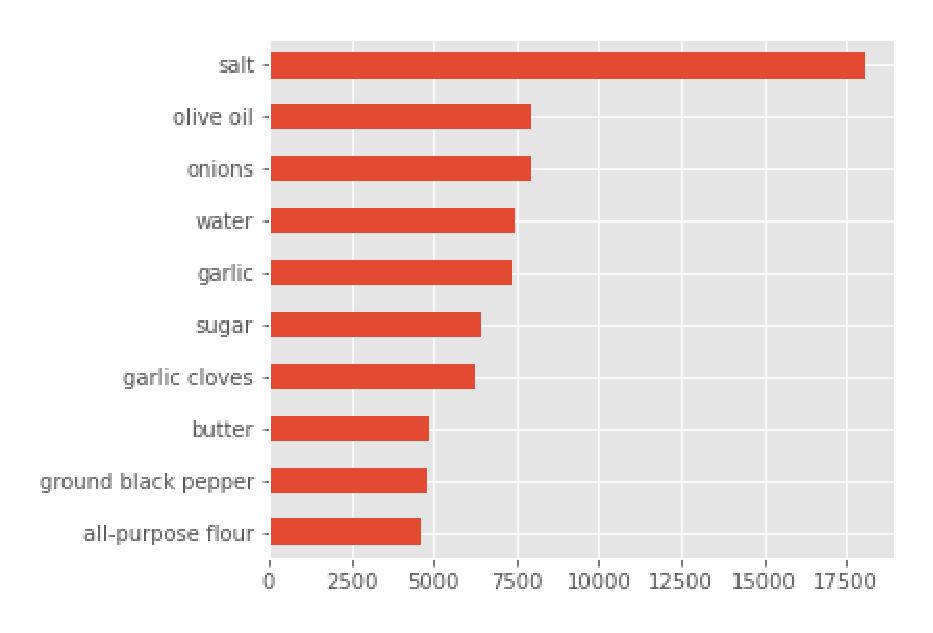
\includegraphics[width=0.5\textwidth]{pic01/cooking.eps} 
      \end{figure}
    }
    \end{center}
  
    \bigskip
    \begin{center}
    
    \end{center}
  \bigskip

\end{slide}
%%
%%==========================================================================================

%%
%%==========================================================================================

%%==========================================================================================

%%==========================================================================================

%%==========================================================================================

%%==========================================================================================

%%==========================================================================================

%%==========================================================================================

 



%%

\begin{slide}{Build Model}
  \begin{center}
  
  
  
  \end{center}
  \bigskip
  \begin{center}
  
  \end{center}
  \bigskip
\end{slide}
%%==========================================================================================


%%
\end{document}

\endinput
